To reach other temperature regimes or to have precise timing control on the introduction of a gas into the chamber, we utilize a Parker Pulse Valve as seen in Figure \ref{fig: general valve}. The pulse valve requires 28 VDC to actuate the solenoid, opening the orifice. The speed at which we operate the pulse valve allows for rise times of milliseconds. During operation of the pulse valve, the PTR is cooling the CBGB components to act as cryopumping surfaces and improve the vacuum in the stem chamber. With appreciable backing pressure ($\approx 1$ atm), the supersonic pulse velocity is defined as:\cite{Pauly}

\begin{equation*}
	v_\infty = \sqrt{\frac{2 k_b T_0}{m}\frac{\gamma}{\gamma - 1}}
\end{equation*}

Where $\gamma$ is the heat capacity ratio $C_p/C_v$, and $T_0$ is the original temperature of the source.

\begin{figure}
	\centering
	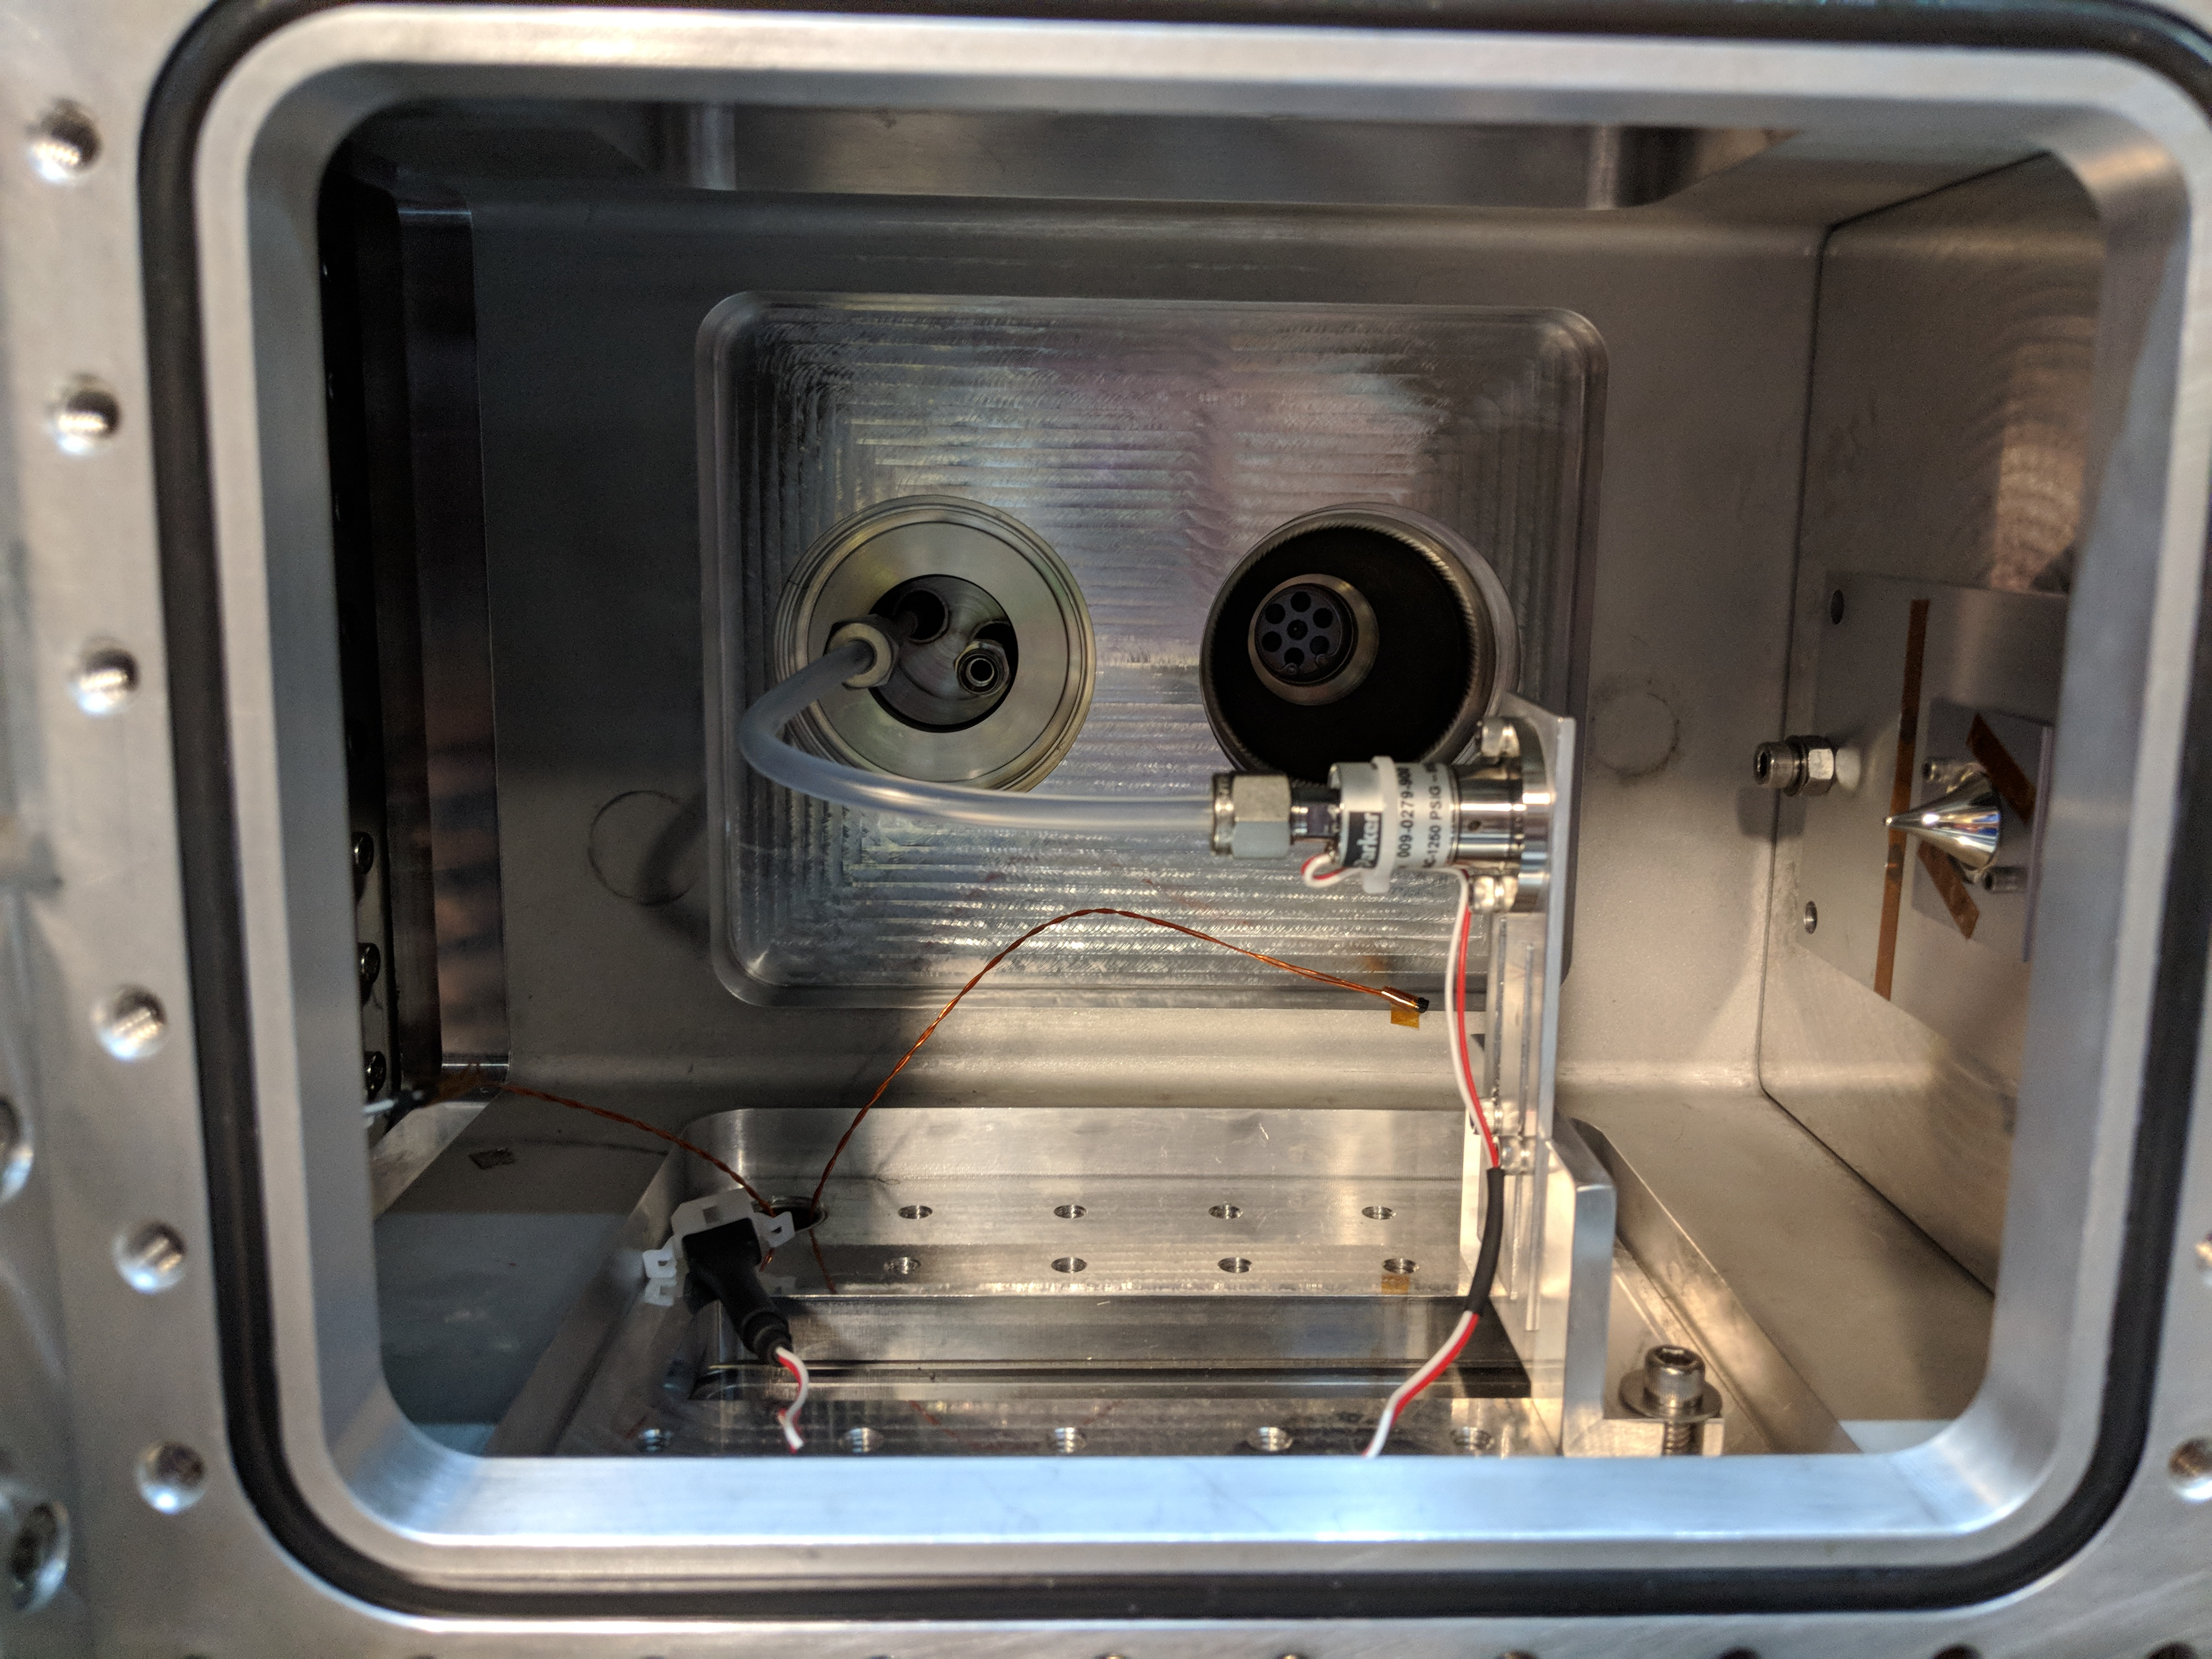
\includegraphics[width=0.8\textwidth]{images/pulse_valve.jpg}
	\caption{Parker Pulse Valve mounted inside the stem chamber aimed at the differential pumping region. The Beam Dynamics skimmer is mounted over the back face of the stem chamber to clean up the supersonic pulse.}
	\label{fig: general valve}
\end{figure}